\documentclass[openany]{article}
\usepackage[a4paper,margin=1in,bottom=1.5in]{geometry}
\usepackage[english]{babel}
\usepackage{tikz}
\usepackage{graphicx}
\usepackage[export]{adjustbox}
\usepackage{fancyhdr}
\usepackage{array} % allow elements of tabular environment to have vertical alignment, e.g., center alignment.

% Configure header in 'titlepage'
\pagestyle{fancy}
\lhead{
\includegraphics[width=4.5cm]{logo_cnpem}}
\rhead{
\includegraphics[width=4cm]{logo_lnls}}
\renewcommand{\headrulewidth}{0pt}
\setlength{\headheight}{52pt}
% Clean footer
\fancyfoot{}

% increase table height factor a little bit (taller cells)
\renewcommand{\arraystretch}{1.5}

%==== Begin DOCUMENT ====
\begin{document}

%--- Begin title page ---
\begin{titlepage}

% Add header to this page
\thispagestyle{fancy}

% Center elements
\begin{center}

\topskip0pt
\vspace*{\fill}
\textbf{\Huge STD-SOE Hardware Manual}\\[20pt]
\textbf{\Huge Version 1.0}\\[20pt]
\textbf{\Huge February/2017}
\vspace*{\fill}

\vfill
\textbf{Beam Diagnostics Group (DIG)}\\[5pt]
\textbf{Brazilian Synchrotron Light Laboratory (LNLS)}\\[5pt]
\textbf{Brazilian Center for Research in Energy and Materials (CNPEM)}
\end{center}

\end{titlepage}
%--- End of title page ---

\newpage
\pagestyle{plain}

%--- About this manual ---
\paragraph{}{\Large\bfseries About this manual}

\paragraph{} This manual is intended for people who need information about the STD-SOE hardware. Information about the timing system structure and operation, firmware, or software can be found in the corresponding manuals.

%--- Table of contents ---
\tableofcontents

\newpage
%--- Section: Hardware Specification ---
\section{Hardware Specification}

\par STD-SOE is a 19 inches 1U module. \\ 110/220V 50/60Hz AC power supply.

% STD-SOE figure
\begin{figure}[!h]
\caption{STD-SOE}
\label{fig:std-soe}
\centering
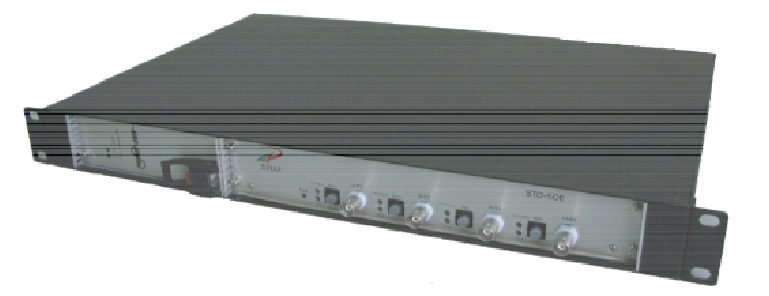
\includegraphics[width=0.7\textwidth]{std-soe-image}
\end{figure}

	% Specification table - Connectors - front panel
	\begin{table}[!h]
	  \centering
	  \caption{STD-SOE front panel connectors}
	  \label{tab:front-panel-connectors}
	  \begin{tabular}{| m{3.5cm} m{4.0cm} m{7.0cm} |}
	    \hline
	    \bfseries Connector & \bfseries Type & \bfseries Description / Specification \\ \hline
	    OUT1 - OUT4 & BNC & Outputs (5.0V TTL level) \\ \hline
	    IN1 - IN4 & HFBR-4531/4532 & Optical Input (Agilent HFBR-2528) \\ \hline
	  \end{tabular}
	\end{table}

	% Specification table - LEDs - front panel
	\begin{table}[!h]
	  \centering
	  \caption{STD-SOE front panel leds}
	  \label{tab:front-panel-leds}
	  \begin{tabular}{| m{3.5cm} m{4.0cm} m{7.0cm} |}
	    \hline
	    \bfseries LED & \bfseries Type & \bfseries Description / Specification \\ \hline
	    PWR & Green LED & Power on \\ \hline
	    TRIGGER1 & Yellow LED & \begin{tabular}{@{}m{6cm}@{}}
				    (On) Uplink established \\
				    (Blink) Trigger output
				    \end{tabular} \\ \hline
	    TRIGGER2 & Yellow LED & \begin{tabular}{@{}m{6cm}@{}}
				    (On) Uplink established \\
				    (Blink) Trigger output
				    \end{tabular} \\ \hline
	    TRIGGER3 & Yellow LED & \begin{tabular}{@{}m{6cm}@{}}
				    (On) Uplink established \\
				    (Blink) Trigger output
				    \end{tabular} \\ \hline
	    TRIGGER4 & Yellow LED & \begin{tabular}{@{}m{6cm}@{}}
				    (On) Uplink established \\
				    (Blink) Trigger output
				    \end{tabular} \\ \hline
	    ITL1 & Red LED & Interlock input activated \\ \hline
	    ITL2 & Red LED & Interlock input activated \\ \hline
	    ITL3 & Red LED & Interlock input activated \\ \hline
	    ITL4 & Red LED & Interlock input activated \\ \hline
	  \end{tabular}
	\end{table}

	% Specification table - Connectors - rear panel
	\begin{table}[!h]
	  \centering
	  \caption{STD-SOE rear panel connectors}
	  \label{tab:rear-panel-connectors}
	  \begin{tabular}{| m{3.5cm} m{4.0cm} m{7.0cm} |}
	    \hline
	    \bfseries Connector & \bfseries Type & \bfseries Description / Specification \\ \hline
	    ITL\_IN\_1 & BNC & Interlock input 1 \\ \hline
	    ITL\_IN\_2 & BNC & Interlock input 2 \\ \hline
	    ITL\_IN\_3 & BNC & Interlock input 3 \\ \hline
	    ITL\_IN\_4 & BNC & Interlock input 4 \\ \hline
	    BYPASS & Switch & Bypass interlock input \\ \hline
	  \end{tabular}
	\end{table}

%--- Section: STD-SOE Hardware ---
\section{STD-SOE Hardware Functions}

	\paragraph{} The STD-SOE module is an Optical to Electrical converter used for converting Timing System triggers. The module has 4 Plastic Optical Fiber inputs (IN1 - IN4) in the front panel. The input signals are converted to 5V TTL level electrical signals, which are output in the corresponding BNC connectors (OUT1 - OUT4). The STD-SOE has 4 independent interlock inputs in the rear panel (ITL\_IN\_1 - ITL\_IN\_4) related to the front panel outputs (OUT1 - OUT4). In order to bypass the interlock inputs, the BYPASS switch (rear panel) can be used.

\end{document}
\grid
